\documentclass{article}

% Language setting
\usepackage[german]{babel}
% Paper Settings
\usepackage[a4paper,top=2cm,bottom=2cm,left=3cm,right=3cm,marginparwidth=1.75cm]{geometry}

% Useful packages
\usepackage{amsmath}
\usepackage{graphicx}
\graphicspath{ {./images/} }
\usepackage[font=small,labelfont=bf]{caption}
\usepackage{blindtext}
\usepackage[colorlinks=true, allcolors=blue]{hyperref}
\usepackage{color,soul}
\usepackage[absolute]{textpos}
\usepackage[onehalfspacing]{setspace}
\usepackage[utf8]{inputenc}
\usepackage{soulutf8}
\usepackage{wrapfig,booktabs}
\usepackage{parskip}

% add and override commands
\newcommand{\estimates}{\overset{\scriptscriptstyle\wedge}{=}} % ≙

% kind of meta, as \maketitle is not in use
\title{Laborbericht 1}
\author{Jannik Hoefener, 2574970}
\date{\today}

\begin{document}
\begin{titlepage}

\begin{textblock*}{188mm}(55mm,20mm)

\includegraphics[height=40mm]{images/hawlogo.png}
\end{textblock*}

\vspace*{\fill}
\begin{center}
    \textsf{\textbf{\Huge Laborbericht 1}} \\
    \vspace*{6mm}
    \textsf{\Huge I/O Ports} \\
    \textsf{\Large Korrektur} % not sure if style is ok...
\end{center}
\vspace*{\fill}

\begin{textblock*}{90mm}(30mm,220mm)
\noindent\textsf{Bericht des ersten Labors eingereicht von} \\
\textsf{Hoefener, Jannik} \\
\textsf{Matrikelnummer 2574970} \\
\textsf{ } \\
\textsf{im Rahmen der Vorlesung Informatik und Elektronik } \\
\textsf{im Studiengang Media Systems} \\
\textsf{am Department Medientechnik der Fakultät DMI} \\
\textsf{an der Hochschule für Angewandte Wissenschaften Hamburg} \\
\textsf{ } \\
\textsf{Lehrender: Prof. Dr. Tessa Taefi} \\
\textsf{Eingereicht am: \today} \\
\end{textblock*}

\end{titlepage}
\newpage
\begin{abstract}
\noindent Diese Dokumentation ist im Rahmen des ersten Labors im Modul „Informatik 3 und Elektronik“ bei Prof. Dr. Tessa Taefi entstanden. All umfassend galt es sich, in Präsens im Labor an der Fachhochschule HAW Hamburg am Campus DMI, mit „Input / Output Ports“ des ATmega328P zu befassen. 
\\
Durch die praktische Umsetzung der gestellten Aufgaben im Labor, war es möglich die gelehrten Inhalte aus den zu vorherigen Vorlesungen umzusetzen und zu reflektieren.  
Infolgedessen wurden tiefergehende Kenntnisse in der Programmiersprache Embedded C, im Microchip Studio und SimulIDE gesammelt. Auch das Verständnis über das Atmel ATmega328P Xplained Mini Board wurde vertieft und verinnerlicht. 
\\
Programmierter Code u den jeweiligen Aufgaben sowie die Verwendeten Grafiken sind im Anhang zu finden. 
Der Anhang wird zusammen mit diesem Bericht als .zip Datei auch über die HAW-Cloud zur Verfügung gestellt:
\\
Cloud Zugang: \href{https://cloud.haw-hamburg.de/index.php/s/XmxVaV3XeUyFTNA}{https://cloud.haw-hamburg.de/index.php/s/XmxVaV3XeUyFTNA} (12345)
\\
\\
Das Labor wurde in Partnerarbeit absolviert, die Berichtserstattung erfolgt jedoch in Einzelarbeit. 
%\hl{Daher ist dieser Bericht aus der Ich-Perspektive geschrieben} 
\\
\\
Gerne darf die Dokumentation zu Präsentationszwecken verwendet werden. 
\end{abstract}

\tableofcontents
\listoffigures
%\listoftables
% quellen sind am ende des Dokumentes
%\bibliographystyle{abbrv}
%\bibliography{sample}

\section{Einleitung}

\noindent Die drei gestellten Aufgaben zum Thema „I/O Ports“ setzen die vermittelten Inhalte aus den entsprechenden Vorlesungen voraus. Auf Basis dieser Kenntnisse und der Umsetzung der Aufgaben, soll durch die Erstellung von Block- und UML Diagrammen, sowie das darauf basierende Schreiben und Debuggen eines korrekten C-Codes, das analytische Verständnis sowie die Planung und Dokumentation des Lösungsansatzes und die letztendliche Implementierung vertieft werden. \\
\\
In der ersten Aufgabe liegt der Fokus auf der Inbetriebnahme des Xplained Mini Boards. \\
In der zweiten Aufgabe soll das selbstentwickelte Shield in Betrieb genommen werden. \\
In der dritten Aufgabe kommt es zur Verwendung von Polling und Interrupts. \\
\\
Final gilt zum Bestehen des Labors eine kurze Abnahme durch Vorstellung der korrekten Aufgabenbearbeitung. \\
\\
%Im Folgenden wird die Aufgabenstellung und Umsetzung dieser detailliert beschrieben.

\section{Materialien und Methoden}

\noindent Für das Schreiben und Debuggen des Programmier-Codes (C) wird die Software Microchip Studio als IDE verwendet.  \\
\\
Als Hardware steht uns Atmel ATmega328P Xplained Mini Board mit und ohne selbstentwickeltem Shield zur Verfügung, welche von der HAW Hamburg zur Verfügung gestellt wird. 
Auf dem Shield ist eine Kingbright LED-Bank (DC-7G3HWA) sowie zwei Buttons verbaut. \\
\\
Alternativ steht uns die Software SimulIDE zu Verfügung, in der man das Verhalten einer bestimmten Hardware simulieren könnte, falls diese zur Verfügung stände.  \\
\\
Des Weiteren wurde die Software Notion während der Bearbeitung verwendet. Hier wurden Code-Text, Bilder und Videos sowie allgemeine Notizen zum Arbeitsprozess gesammelt und strukturiert. \\
\\
Für die Erstellung der UML-Diagramme wurde die Software diagrams.net (draw.io) verwendet.  
Für die Erstellung der Schaltbilder wurde die Software easyEDA verwendet, welche für den Labor Bericht zwingend notwendig ist.  \\
\\
Geschrieben und gerendert wurde der Bericht in LaTeX. Hier für wurde eine Vorlage von Sören Helms verwendet.\\

\section{Aufgabenstellungen und Umsetzung}

\subsection{Aufgabe 1: Inbetriebnahme des Xplained Mini Board}

In der ersten Aufgabe liegt der Fokus auf der Inbetriebnahme des Xplained Mini Boards.
\\
Es soll die in der zweiten Vorlesung gestellte Hausaufgabe „LEDOnButtonPress“ auf dem Xplained Mini Board zum Laufen gebracht werden. \\  
\\
Anschließend soll auf Basis dieser ein neues Programm „CountButtonAndBlink“ geschrieben werden. Ziel soll es sein, fortlaufend eine LED so häufig blinken zu lassen, wie ein Button gedrückt wurde.
\\
Das folgende Blockdiagramm (Abbildung \ref{fig:bd-a1}) und Schaltbild (Abbildung \ref{fig:sb-a1}) stellen den Zusammenhang zwischen dem Input, dem Microcontroller und dem Output im Programm CountButtonAndBlink dar. Die LED ist auf Port B5 und der Button auf Port B7 verbunden.\\

\begin{figure}[htb]
    \centering
    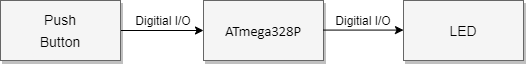
\includegraphics[width=0.75\textwidth]{images/A1-BD-CountButtonAndBlink.d.png}
    \caption{Blockdiagramm \textit{CountButtonAndBlink}}
    \label{fig:bd-a1}
    % Quellenangabe: Eigene Darstellung per Diagrams.net
\end{figure}

\begin{figure}[htb]
    \centering
    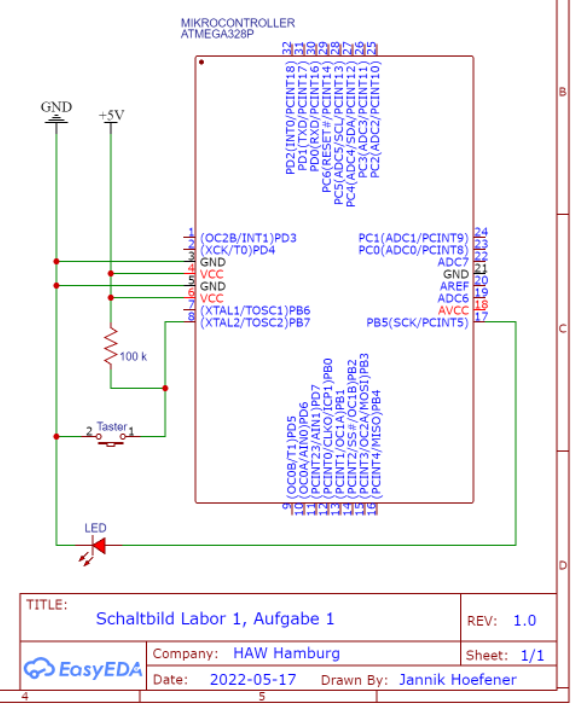
\includegraphics[width=0.5\textwidth]{images/A1-Schaltbild.png}
    \caption{Schaltbild \textit{CountButtonAndBlink}}
    \label{fig:sb-a1}
    % Quellenangabe: Eigene Darstellung per EasyEDA
\end{figure}

\noindent Das Aktivitätsdiagramm (Abbildung \ref{fig:ad-a1}) beschreibt die Abfolge der Prozesse des Programms CountButtonAndBlink. Wenn der Knopf gedrückt wurde, blinkte die LED im Anschluss so oft auf, wie sie zuvor gedrückt wurde. 

\begin{figure}[ht]
    \centering
    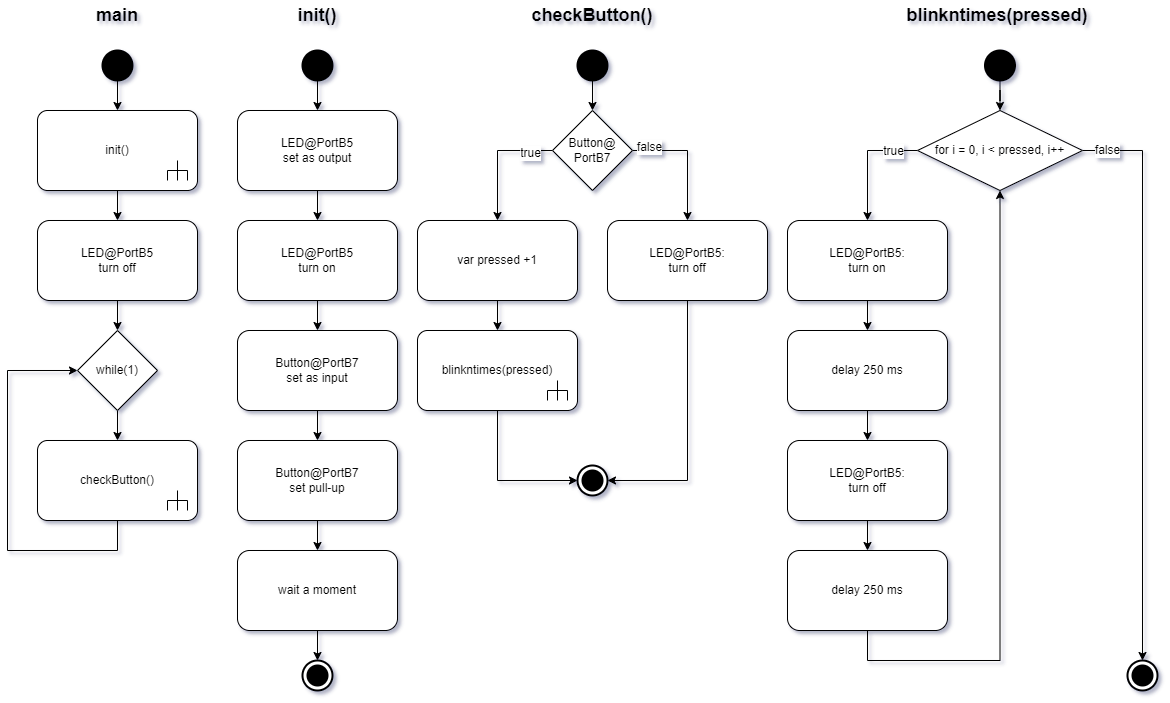
\includegraphics[width=\textwidth]{images/A1-AD.png}
    \caption{Aktivitätsdiagramm \textit{CountButtonAndBlink}}
    \label{fig:ad-a1}
    % Quellenangabe: Eigene Darstellung per Diagrams.net
\end{figure}

\subsection{Aufgabe 2: Inbetriebnahme des Shields}

\noindent In der zweiten Aufgabe soll das selbstentwickelte Shield in Betrieb genommen werden.

\subsubsection{Teilaufgabe A: Stromversorgung}

\noindent Hierfür soll zuerst ermittelt werden, ob die Ports die LEDs mit ausreichend Strom versorgen.\\

%\begin{figure}[htb]
%    \centering
%    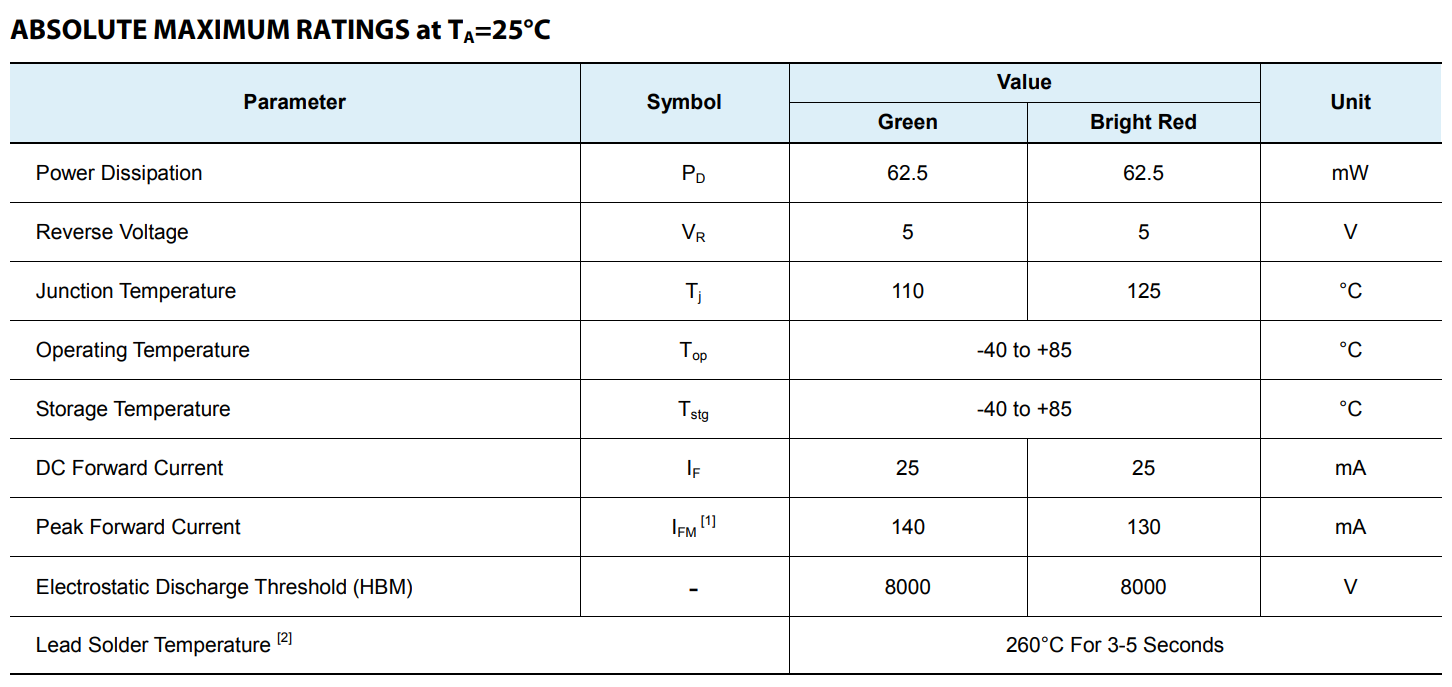
\includegraphics[width=0.75\textwidth]{images/tabelle-kingbright-neu.png}
%    \caption{Datenblatt: LED-Bank, Quelle: \cite{Kingbright}}
%    \label{fig:datenblatt-kingbright}
%\end{figure}
\\
\noindent Mit der Formel für die Berechnung der Stromstärke \(I = \frac{U}{R}\) lässt sich der benötigte Strom für eine LED berechnen, wobei 5V die Spannung auf dem Board ist, 2,3V die Spannung der LED und \(220  \Omega\) der Widerstand vor dem LED Array ist. Die Werte sind den Datenblättern \cite{AtmelDatasheet,Kingbright} entnommen.

\begin{equation}
    I = \frac{(5V-2,3V}{220 \Omega} = 12,27 mA
    \label{eq:einzelneLed}
\end{equation}

\begin{equation}
    10 \times 12,27 mA = 122,7 mA
    \label{eq:ledBank}
\end{equation}

\noindent Entsprechend der Formel \ref{eq:einzelneLed} beträgt der Strom für eine einzelne LED 12,27 mA und der Strom für alle zehn LEDs 122,7 mA, siehe Formel \ref{eq:ledBank}. 

\begin{figure}[htb]
    \centering
    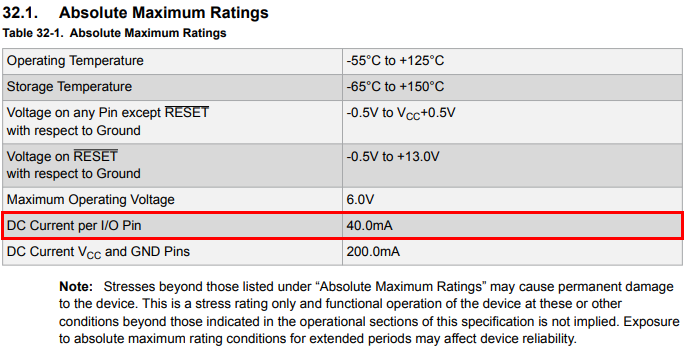
\includegraphics[width=0.75\textwidth]{images/tabelle-atmega.png}
    \caption{Datenblatt ATmega328P, Quelle: \cite{AtmelDatasheet}}
    \label{fig:datenblatt-atmega}
\end{figure}

\noindent Laut dem Datenblatt des ATmega328P (Abbildung \ref{fig:datenblatt-atmega}) ist die maximale Stromstärke pro I/O Pin 40 mA. Somit können alle LEDs problemlos mit Strom versorgt werden, da jede LED mit einem eigenen I/O Pin verbunden ist.

\subsubsection{Teilaufgabe B: Portierung der ersten Aufgabe}

\noindent Anschließend soll mit Hilfe des Programms „LEDOnButtonPress“ und dem selbstentwickelten Shield, Button 1 so angesteuert werden, dass dieser bei Tastendruck die erste grüne LED zum Blinken bringt.
\\
\\
Das folgende Blockdiagramm (Abbildung \ref{fig:bd-a2b}) und Schaltbild (Abbildung \ref{fig:sb-a2b}) stellen den Zusammenhang zwischen dem Input, dem Microcontroller und dem Output im Programm LEDOnButtonPress dar. Die LED sitzt nun auf Port C1 und der Button auf Port D1. \\

% adding a page just for figures

\begin{figure}[htb]
    \centering
    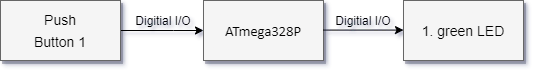
\includegraphics[width=0.7\textwidth]{images/A2b-BD-LEDOnButtonPressmitShield.d.png}
    \caption{Blockdiagramm \textit{LEDOnButtonPress}}
    \label{fig:bd-a2b}
    % quelle?
\end{figure}

\begin{figure}[htb]
    \centering
    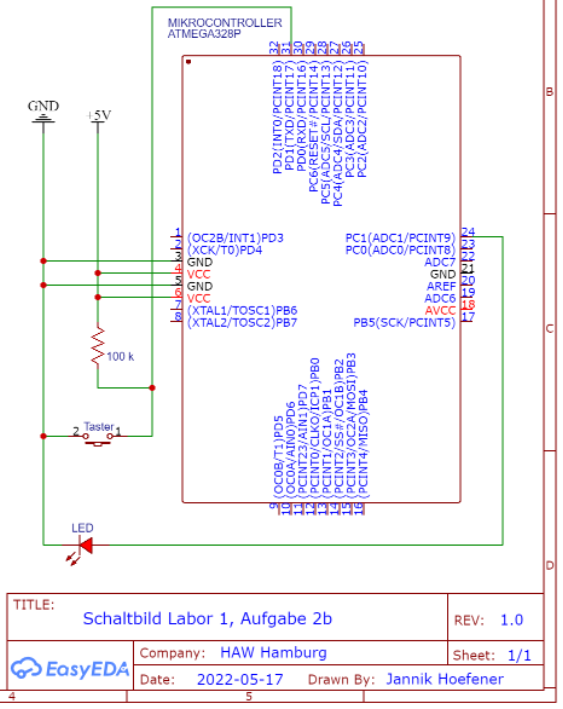
\includegraphics[width=0.5\textwidth]{images/A2b-Schaltbild.png}
    \caption{Schaltbild \textit{LEDOnButtonPress}}
    \label{fig:sb-a2b}
    % quelle?
\end{figure}

\newpage
\vfill

\begin{figure}[]
    \centering
    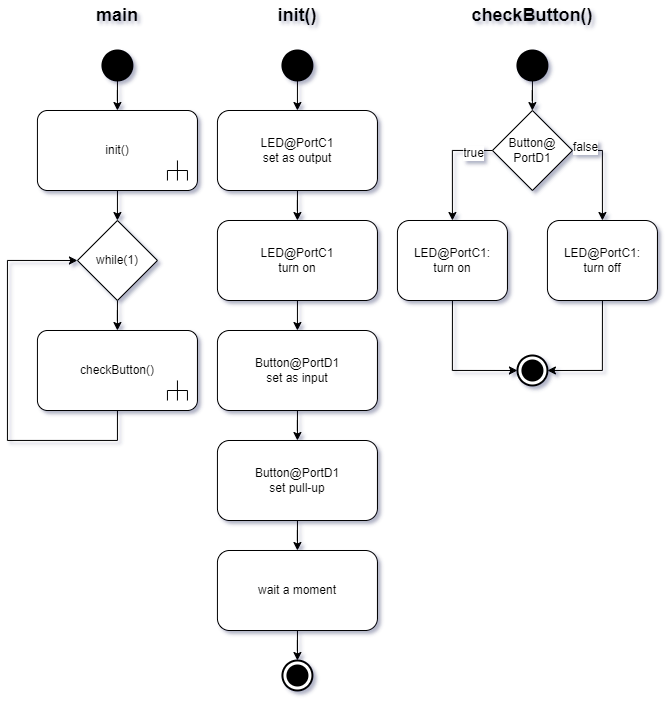
\includegraphics[width=0.7\textwidth]{images/A2b-AD.png}
    \caption{Aktivitätsdiagramm \textit{LEDOnButtonPress}}
    \label{fig:ad-a2b}
    % quelle: Eigene Erstellung: 
\end{figure}

\vfill

\noindent Entsprechend zugrundeliegenden Aufgabe ohne Shield haben wurde der alte Code genommen, die I/O Pins aus dem oberen Bereich des Codes (define …) angepasst und den fertigen Code auf das Board hochgeladen. Wie erwartet wurde das gleiche Programm nur auf anderen Pins auf dem Shield angezeigt, beziehungsweise musste der Knopf auf dem Shield gedrückt werden.
Die Abfolge der Prozesse des Programms wird im folgendem Aktivitätsdiagramm (Abbildung \ref{fig:ad-a2b}) dargestellt.

\clearpage

\subsubsection{Teilaufgabe C: Die Wirkung des Pullup Widerstandes}

\noindent Es gilt nun zu beobachten, wie sich das Programm verhält, wenn der Pullup Widerstand des Push-Buttons entfernt wird.
\\
\\ Ein Pull-Down verbindet den Button so mit Ground, dass nichts anliegt, wenn der Knopf offen ist und 5V anliegen, wenn der Knopf gedrückt wird. 
\\ Pull-Up legt 5V an, wenn der Knopf offen ist und auf Ground, sobald der Knopf gedrückt wird.
\\
\\ Es lässt sich die Zeile, in der der Internal Pull Up eingeschaltet ist, löschen und das Programm neu auf das Board laden.
\\
\\
Wie zu erwarten, gibt es Probleme bei der Erkennung, ob der Button gedrückt ist, denn die LED leuchtet dauerhaft. Vermutlich wird der Knopf immer als gedrückt erkannt. 
Wird der Pull-Up wieder eingefügt, funktioniert das Programm wieder, wie es soll.

\subsubsection{Teilaufgabe D: Blinken mit Reset}

\noindent Das Programm soll nun um einen zweiten Button erweitert werden. Dieser soll bei Knopfdruck die Anzahl der Blinks zurück setzten. Dies wird im Folgenden Blockdiagramm (Abbildung \ref{fig:bd-a2d}) dargestellt.\\

\begin{figure}[htb]
    \centering
    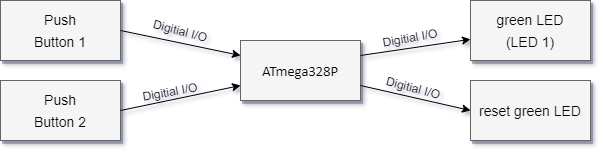
\includegraphics[width=0.75\textwidth]{images/A2d-BD-LEDOnButtonPressmitErweiterungumButton2.d.png}
    \caption{Blockdiagramm \textit{LEDOnButtonPress mit zwei Buttons}}
    \label{fig:bd-a2d}
    % quelle?
\end{figure}

\noindent Aus der bisherigen checkButton() Funktion wurden zwei neue Funktionen erstellt. Die eine prüft nach Button1 der die Blinks erhöhen (inkrementieren) soll, die andere nach Button2 die die Blinks auf 0 setzen (resetten) soll. Entsprechend wurden die Funktionen benannt. Dies ist im folgenden Aktivitätsdiagram (Abbildung \ref{fig:ad-a2d}) erkenntlich.

\begin{figure}[htb]
    \centering
    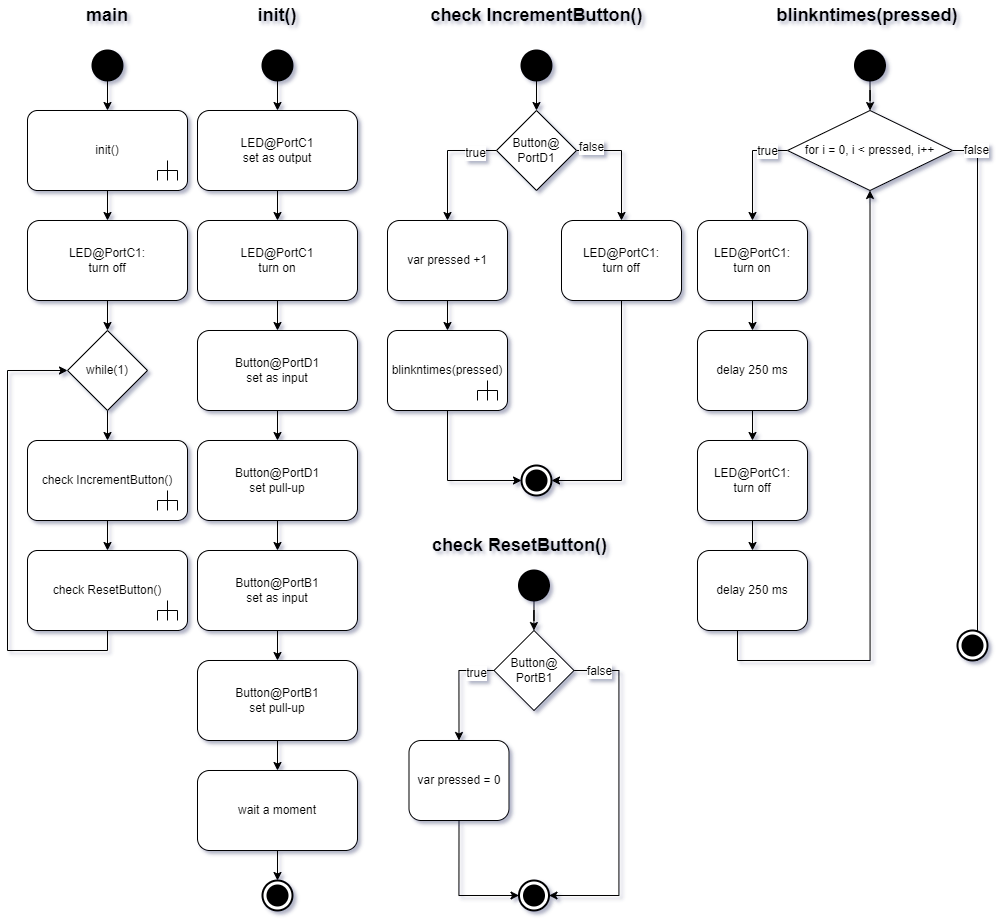
\includegraphics[width=0.95\textwidth]{images/A2d-AD.png}
    \caption{Aktivitätsdiagramm \textit{LEDOnButtonPress mit zwei Buttons}}
    \label{fig:ad-a2d}
    % quelle?
\end{figure}

% bisschen erzwungene ordnung
\newpage

\subsubsection{Teilaufgabe E: BlinkDual}

\noindent Final soll das Programm so verändert werden, dass fortlaufend je Tastendruck die passende Zahl in binär auf der LED-Bank angezeigt wird. Dabei ist die maximal darstellbare Zahl die 15 in binär. 

\noindent Das folgende Blockdiagramm (Abbildung \ref{fig:bd-a2e}) und Schaltbild (Abbildung \ref{fig:sb-a2e}) stellen den Zusammenhang zwischen dem Input, dem Microcontroller und dem Output im Programm CountButtonDualBlinkShield dar.

\noindent Dem folgenden Aktivitätsdiagramm (Abbildung \ref{fig:ad-a2e}) ist das zuvor beschriebene Verhalten des Programms zu entnehmen. 
\\Des Weiteren wird durch Modulo 16 sichergestellt, dass die Counter Variable im gewünschten Bereich bleibt und somit nach 15 wieder bei 0 anfängt zu zählen.
\\Beim drücken des Button 2 wird ein Reset des Zählers ausgeführt.\\

\begin{figure}[!htb]
    \centering
    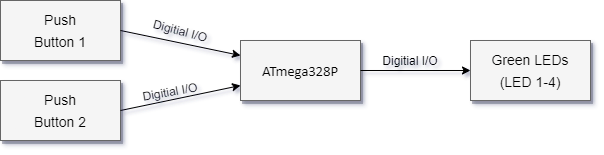
\includegraphics[width=0.75\textwidth]{images/A2e-BD-LEDOnButtonPressmitErweiterungumButton2dual.d.png}
    \caption{Blockdiagramm \textit{LEDOnButtonPress (dual) mit zwei Buttons}}
    \label{fig:bd-a2e}
    % quelle?
\end{figure}

\begin{figure}[htb]
    \centering
    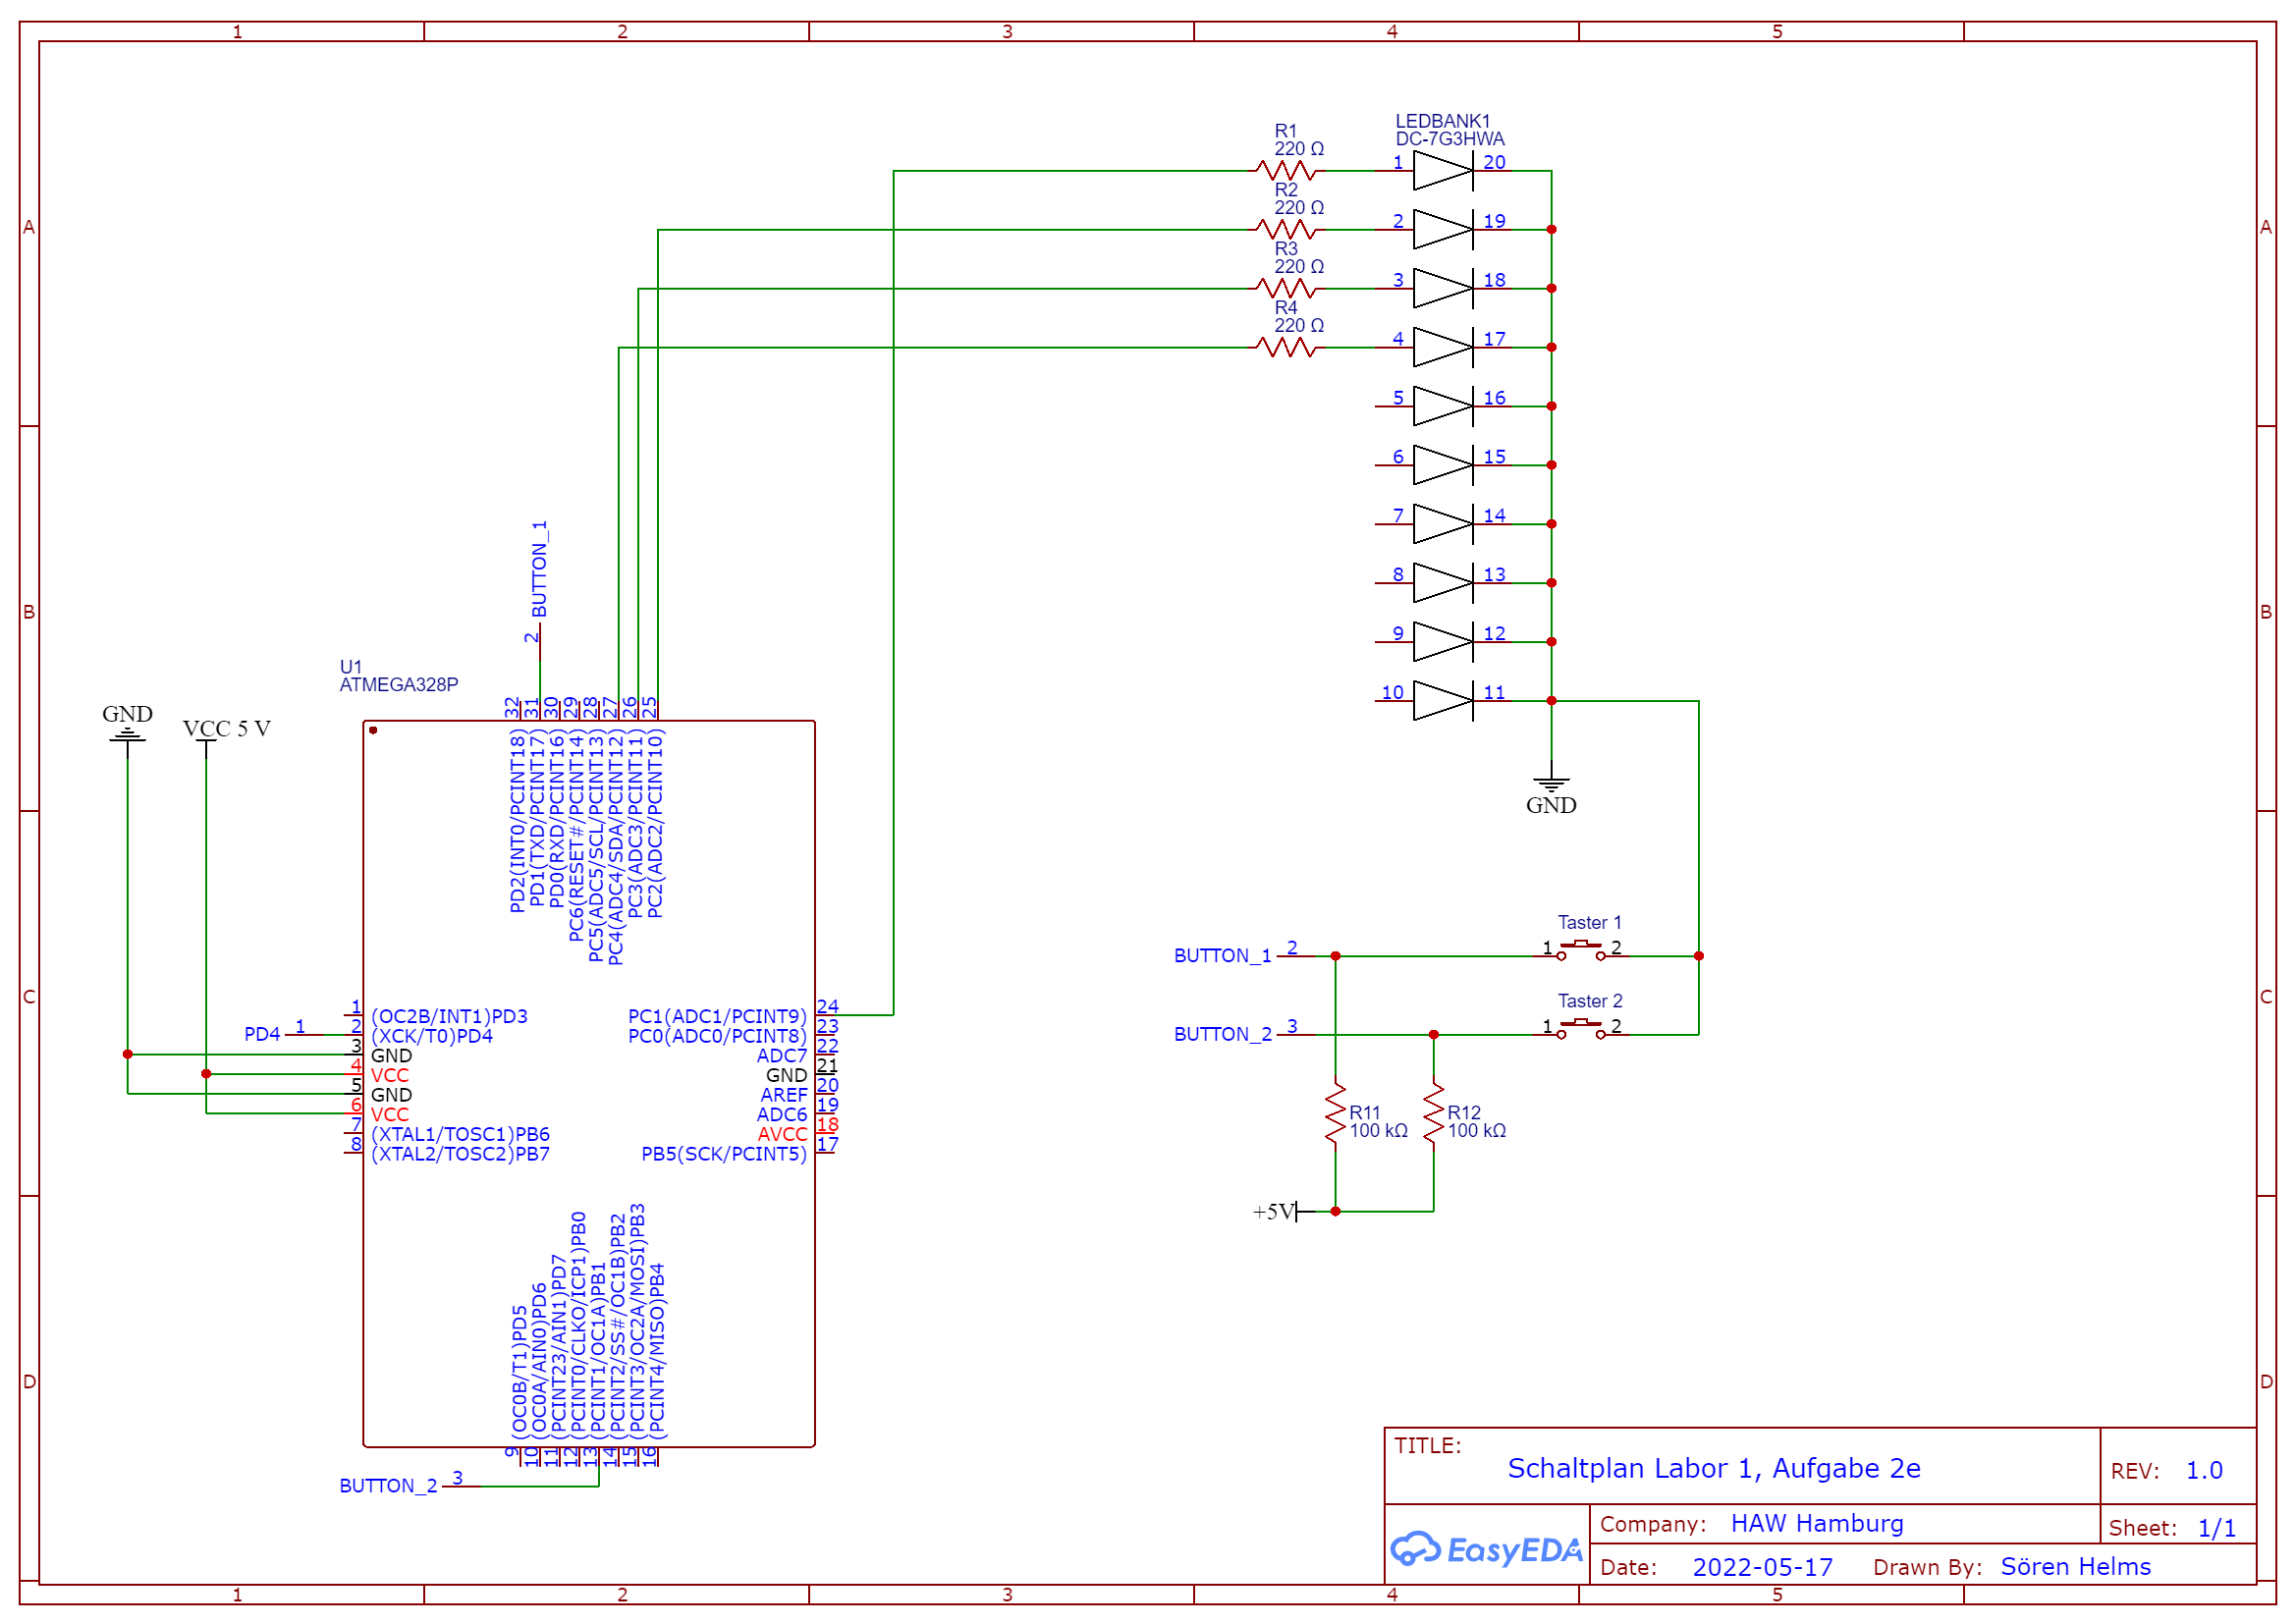
\includegraphics[width=\textwidth]{images/A2e-Schaltbild.png}
    \caption{Schaltbild \textit{LEDOnButtonPress (dual) mit zwei Buttons}, Quelle: \cite{SchaltbilderS}}
    \label{fig:sb-a2e}
\end{figure}

\begin{figure}[htb]
    \centering
    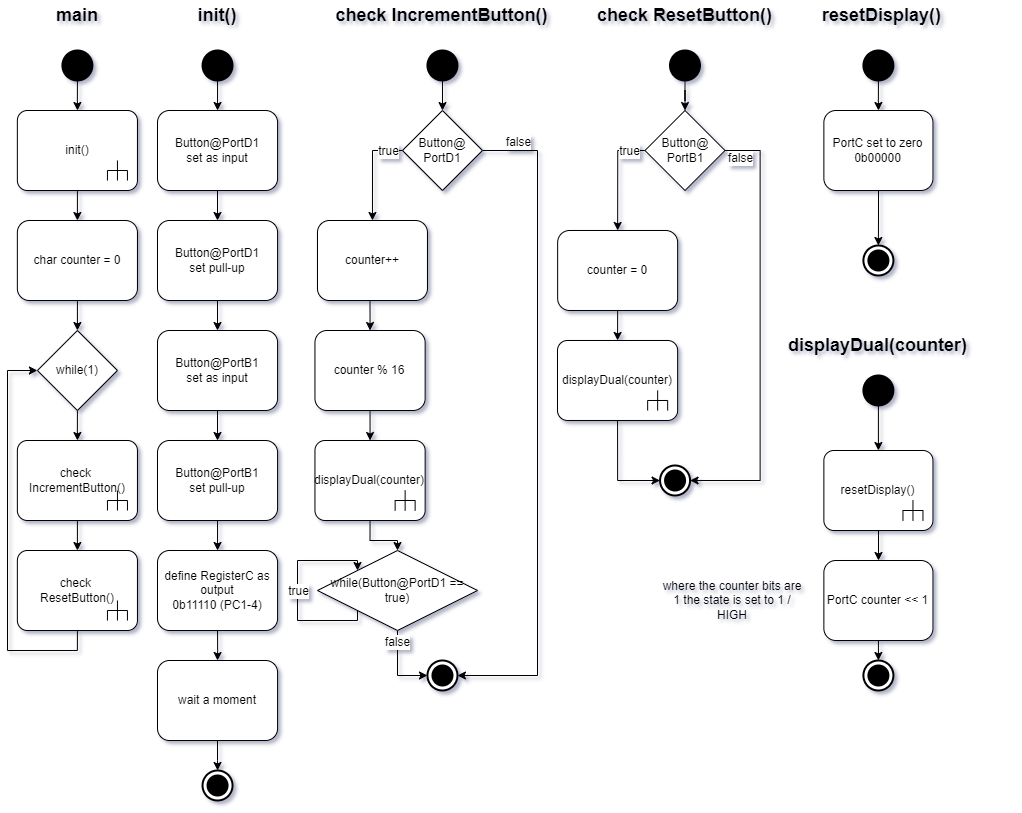
\includegraphics[width=\textwidth]{images/A2e-AD.png}
    \caption{Aktivitätsdiagramm \textit{LEDOnButtonPress (dual) mit zwei Buttons}}
    \label{fig:ad-a2e}
    % quelle?
\end{figure}

% Abschnittsumbruch - floats müssen bis hierhin eingebunden sein, dürfen nicht dahinter gezaubert werden.
\clearpage

\subsection{Aufgabe 3: Verwendung von Interrupts}

In der dritten Aufgabe kommt es zur Verwendung von Polling und Interrupts.
\\
\\ 
Dafür sollen bei gehaltenem Knopfdruck, je nach Knopf, jeweils die sieben grünen LEDs oder die drei roten LEDs zum Leuchten gebracht werden.
\\
\\ Das folgende Blockdiagramm (Abbildung \ref{fig:db-a3}) und Schaltbild (Abbildung \ref{fig:sb-a3}) stellen den Zusammenhang zwischen dem Input, dem Microcontroller und dem Output dar. 
%stellen den Zusammenhang zwischen Input und Output an dem Microcontroller dar.
\\ 
\\ 
\begin{figure}[htb]
    \centering
    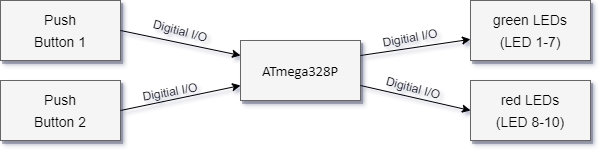
\includegraphics[width=0.75\textwidth]{images/A3-BD-Interrupts.d.png}
    \caption{Blockdiagramm \textit{Green/Red LEDs ansteuern mit zwei Buttons}}
    \label{fig:db-a3}
    % quelle?
\end{figure}

\begin{figure}[ht]
    \centering
    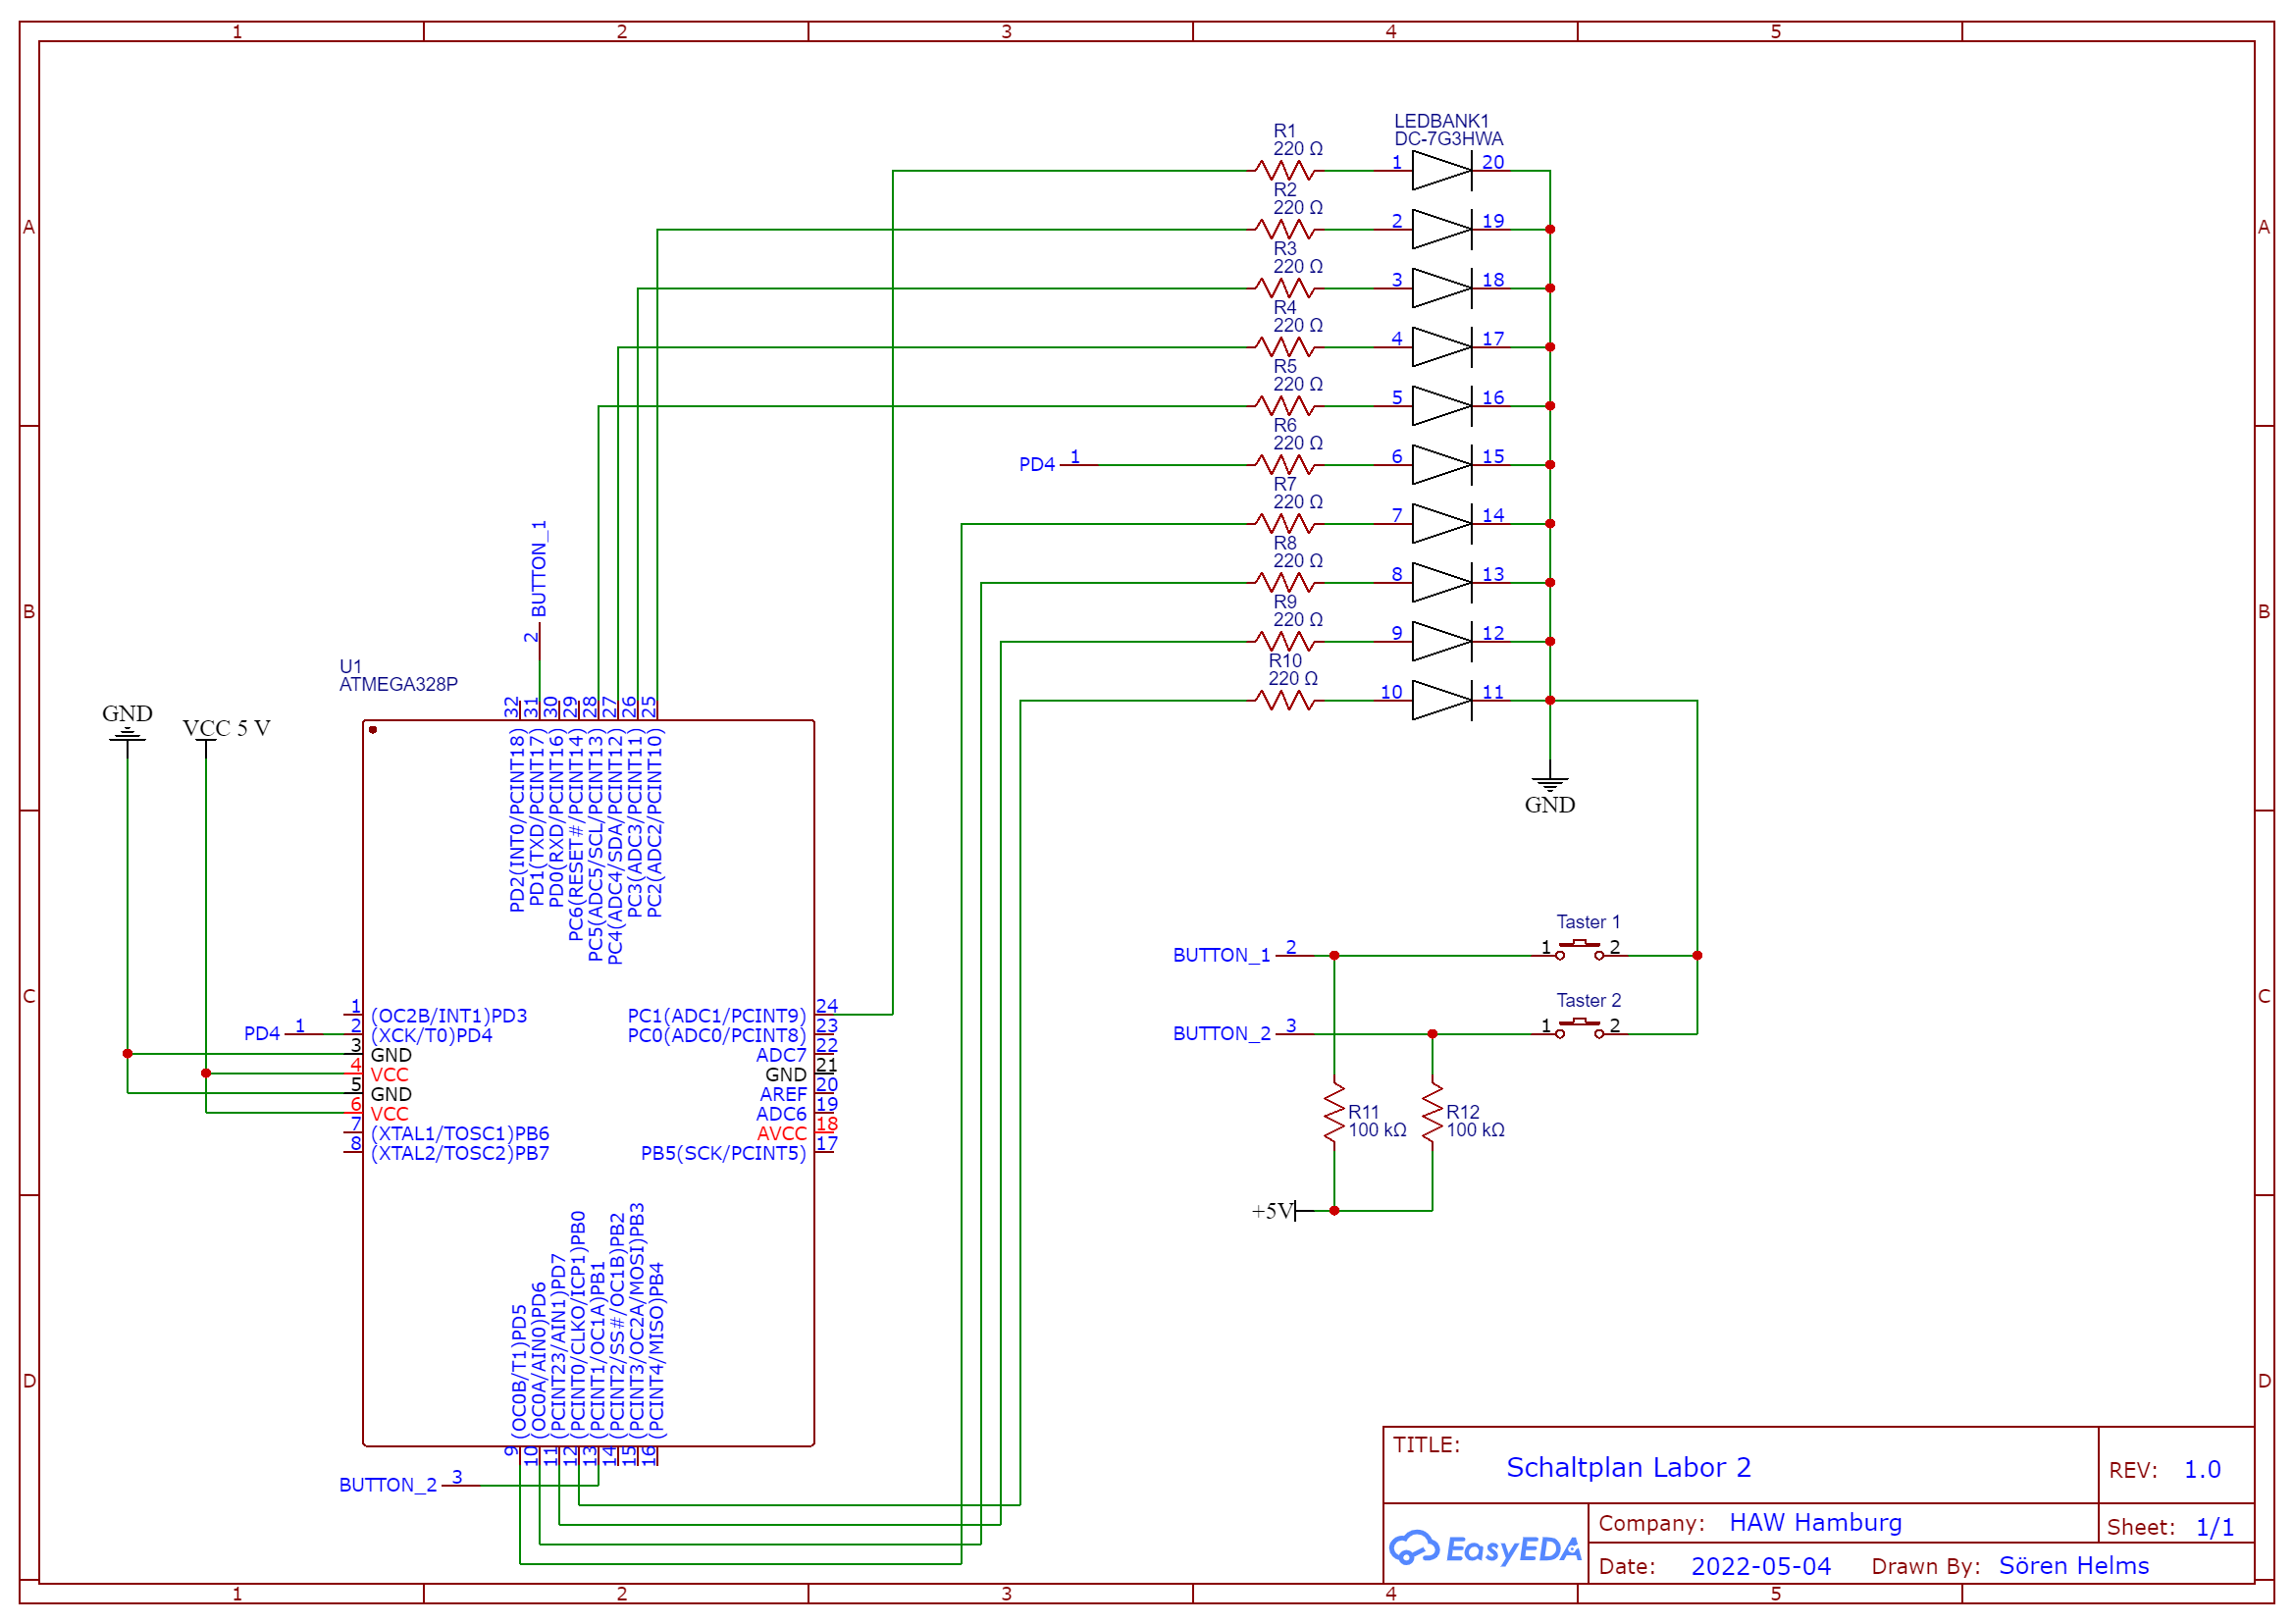
\includegraphics[width=\textwidth]{images/A3-Schaltbild.png}
    \caption{Schaltbild \textit{Green/Red LEDs ansteuern mit zwei Buttons}, Quelle: \cite{SchaltbilderS}}
    \label{fig:sb-a3}
\end{figure}

\subsubsection{Teilaufgabe A: Polling}

\noindent Zuerst sollte dies mit Polling (ständige Statusabfrage) umgesetzt werden.
Diese Herangehensweise stellt das folgende Aktivitätsdiagram (Abbildung \ref{fig:ad-a3a}) dar. 

\begin{figure}[ht]
    \centering
    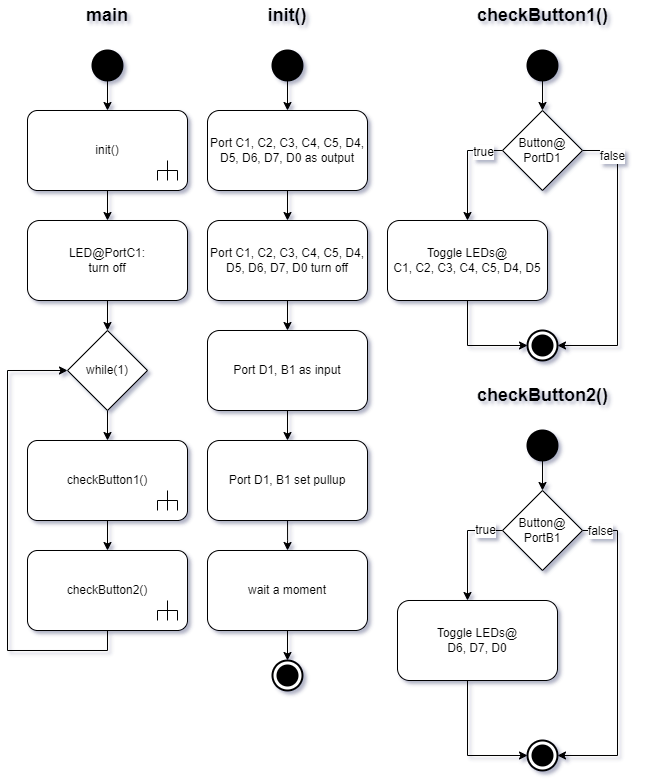
\includegraphics[width=0.75\textwidth]{images/A3a-AD-Polling.png}
    \caption{Aktivitätsdiagramm \textit{Green/Red LEDs ansteuern mit zwei Buttons per Polling}}
    \label{fig:ad-a3a}
    % quelle?
\end{figure}

\subsubsection{Teilaufgabe B: Interrupts}

\noindent Anschließend soll das Polling durch die Verwendung von Interrupts abgelöst werden, wobei bei Button 1 ein Pin-Change Interrupt und bei Button 2 ein externes Interrupt verwendet werden soll, wie im Aktivitätsdiagram (Abbildung \ref{fig:ad-a3b}) dargestellt.
Kommt es zu einem PinChange Interrupt an Port B leuchten die grünen LEDs, kommt es dagegen zu einem externen Interrupt an Port D so leuchten die roten LEDs.

\begin{figure}[ht]
    \centering
    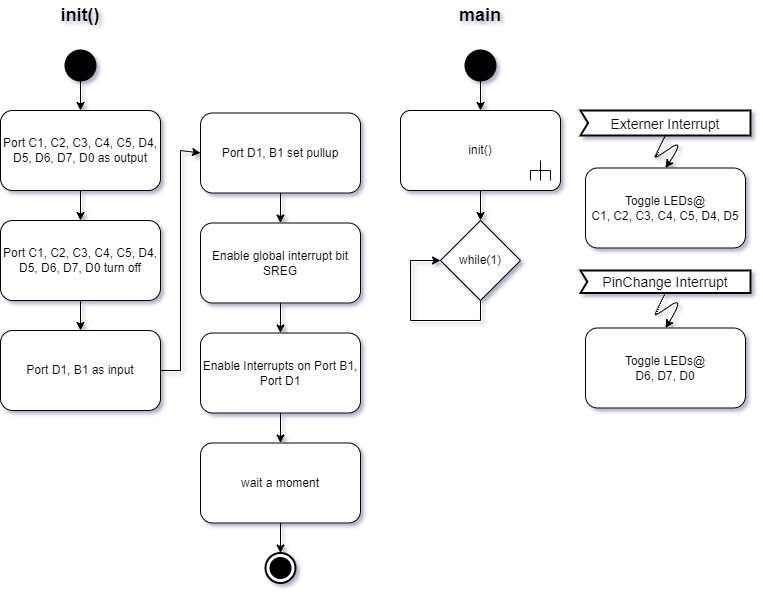
\includegraphics[width=0.75\textwidth]{images/A3b-AD-Interrupt.png}
    \caption{Aktivitätsdiagramm \textit{Green/Red LEDs ansteuern mit zwei Buttons per Interrupts}}
    \label{fig:ad-a3b}
    % quelle?
\end{figure}

\clearpage

\section{Fazit}

% \noindent Disclaimer: Im folgenden Fazit beziehe ich mich auf uns als Team, als auch auf mich allein.
\\
Abschließend lässt sich sagen, dass trotz großer Anstrengung, aufgrund von Zeitmangel und einem hohen Arbeitsumfang, das Labor sich als sehr lehrreich herausgestellt hat. 
\\
\\
Es traten einige Probleme auf wie beispielsweise dass bei uns die SimulIDE nicht funktionierte, sodass bedauerlicherweise keine zuvor getestete und funktionierende Version ins Labor mitgenommen werden konnte.
\\
Doch auch für den Wissensstand, den ich mitbrachte, war am Ende das Labor so umfangreich, dass ich zwei weitere Nachbearbeitungstermine zur Vollständigen Aufbereitung des Labors brauchte.   
\\
\\
Daher nehme ich mir für das nächste Labor vor, nochmal grundlegend die Inhalte der Vorlesung sowie die Funktionsweise der Microcontroller Programmierung aufzuarbeiten und eine all umfassende Übersicht zu verschaffen.  
\\
\\
Wir als Team nehmen uns für das nächste Labor vor, die Diagramme vorzubereiten, sodass das Grundlegende Design schon fertig vorliegt, um mehr Zeit für die Implementierung zu haben.

Zusammenfassend kann also gesagt werden, dass die Durchführung dieses Labors nicht einfach gewesen ist. Es wurde durch Fehler und Schwierigkeiten gelernt und eine neue Motivation aufgebaut, diesen Problemen in Zukunft schon vorher entgegenzuwirken.

\bibliographystyle{abbrv}
\bibliography{sample}

\section*{Eigenständigkeitserklärung}

\noindent Hiermit versichere ich, dass ich das vorliegende Dokument selbständig und nur mit den angegebenen Hilfsmitteln verfasst habe. Alle Passagen, die ich wörtlich aus der Literatur oder aus anderen Quellen wie z. B. Internetseiten übernommen habe ich deutlich als Zitat mit Angabe der Quelle kenntlich gemacht. 
\\
\\
\\
\\
Ort, Datum
\\
\\
\\
\\
Unterschrift

\end{document}